%!TEX root = lec08_nosql.tex

%
% ------------------------------------------------------------------------------------------------------------
%

\begin{frame}{Key/Value Stores}

Key/Value stores have become popular recently. Example systems include Apache HBASE, Amazon's DynamoDB and Google's BigTable.

\vskip1em

\begin{center}
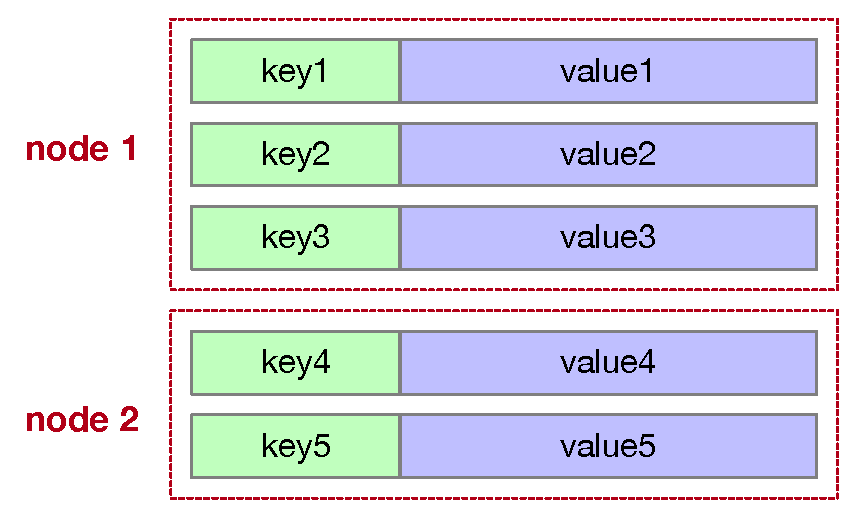
\includegraphics[width=0.5\textwidth]{figures/key_value_store.eps}
\end{center}

\vskip1em

Fundamentally, these systems implement \alert{partitioned tables} as discussed before with the added restriction that \alert{the partition is defined on a singleton key attribute}.
\end{frame}


%
% ------------------------------------------------------------------------------------------------------------
%

\begin{frame}{Why are Key/Value Stores So Popular?}

Except for the keys, each tuple can have its own ``schema'', with its own columns. Also, the ``columns'' can store non-1NF data, like arrays and lists or other data structures.

In other words, these key/value stores are good for storing \textbf{semistructured data}!

\vskip1em
Example:

\begin{center}
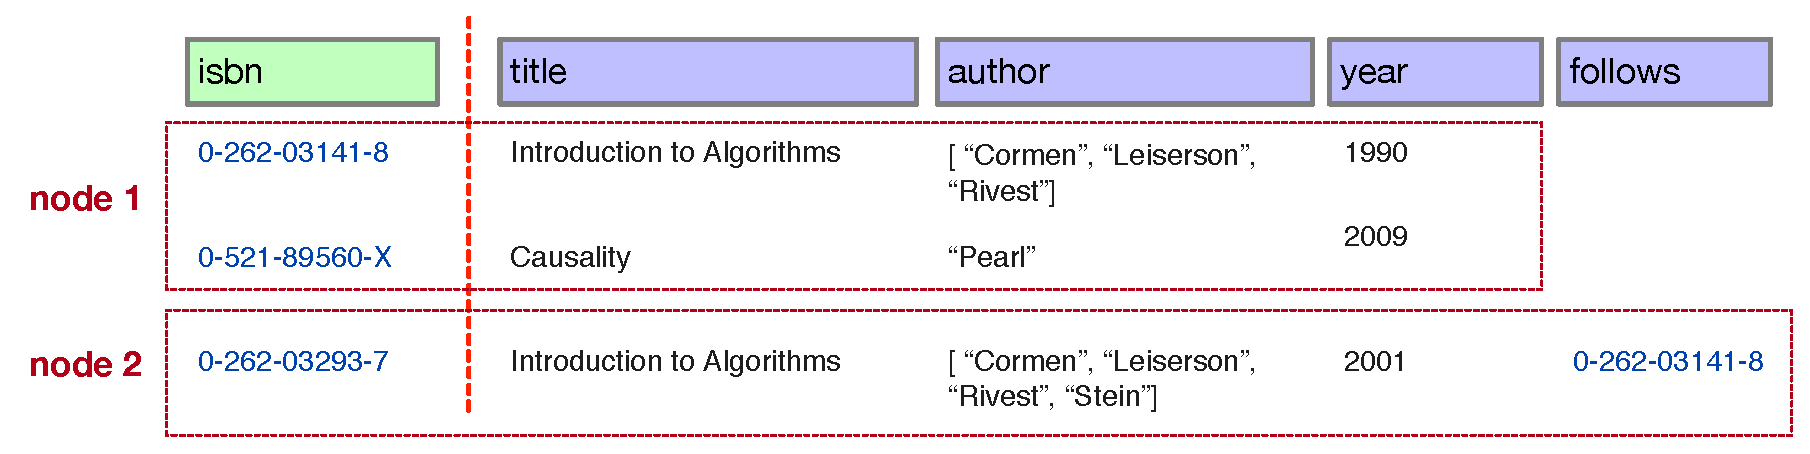
\includegraphics[width=1\textwidth]{figures/key_value_store_example.eps}
\end{center}
\end{frame}

%
% ------------------------------------------------------------------------------------------------------------
%

\begin{frame}

\begin{center}
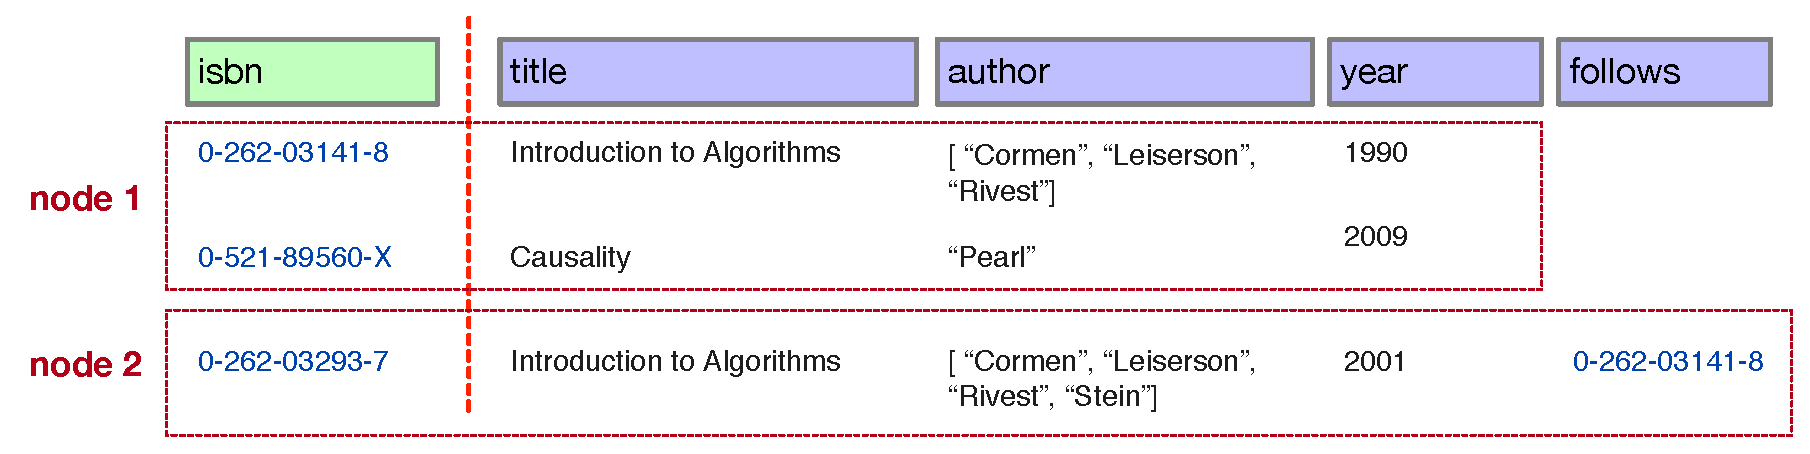
\includegraphics[width=1\textwidth]{figures/key_value_store_example.eps}
\end{center}

\vskip1em

\alert{\textbf{Support for application-level constraints}}?
\begin{itemize}[-,topsep=-5pt]
\item ex: every ISBN in a ``follows'' attribute must match an ISBN of some other ``row'' in the table.
\end{itemize}
 
\vskip1em

The programmer is on their own here... in general, key/value stores \textbf{do not support} constraints like foreign keys. In fact, they don't even support triggers easily.
\end{frame}


%
% ------------------------------------------------------------------------------------------------------------
%

\begin{frame}

Many ``document stores'' are just key-value stores under the hood, where the \textbf{\alert{keys are system-generated}} at insertion time.

These systems allow programs to \textcolor{blue}{C}reate, \textcolor{blue}{R}ead, \textcolor{blue}{U}pdate, or \textcolor{blue}{D}elete objects (\textcolor{blue}{CRUD}).

\vskip2em

\begin{columns}[onlytextwidth]
\begin{column}{0.75\textwidth}
Systems like Elasticsearch also automatically populate indexes as documents are loaded to the ``table''. For example, Elasticsearch indexes allow it to very quickly find documents that match phrases or keywords provided by the user or an application, even for very large collections.
\end{column}
\qquad\begin{column}{0.25\textwidth}
\includegraphics[width=1\textwidth]{figures/elastic.png}
\end{column}
\end{columns}

\vskip1em

CMPUT361 covers those kinds of indexes and a lot more about document processing.
\end{frame}

%
% ------------------------------------------------------------------------------------------------------------
%

\begin{frame}[fragile]

\vskip1em

Example: storing document into an Elasticsearch ``table'' \lstinline!books!:

\vskip1em

\bgroup
\lstset{basicstyle=\ttfamily\scriptsize}

\begin{lstlisting}
POST books/_doc/
{
    "isbn" : "0-262-03141-8",
    "title" : "Introduction to Algorithms",
    "year" : 1990, 
    "authors" :  [ "Cormen", "Leiserson", "Rivest"]
}
\end{lstlisting}
 
Sample output:

\begin{lstlisting}
{
    "_shards" : { "total" : 2, "failed" : 0, "successful" : 2 },
    "_index" : "books",
    "_type" : "_doc",
    -:"_id" : "W0tpsmIBdwcYyG50zbta":-,
    "_version" : 1,
    "_seq_no" : 0,
    "_primary_term" : 1,
    "result": "created"
}\end{lstlisting}

\egroup
\end{frame}

%
% ------------------------------------------------------------------------------------------------------------
%

\begin{frame}{Consistent Hashing}

Consistent hashing is a key ingredient in distributed key/value stores that allows for load balancing even when nodes join or leave the system.

\vskip1em

\begin{columns}[onlytextwidth]
\begin{column}{0.6\textwidth}
Nodes (A, B, C, and D) and objects (1, 2, 3, ...) are hashed to the same circular space (e.g., 32bit hash values with wraparound).

\vskip1em

Objects are assigned to the \textbf{closest} available node in the system.
\end{column}
\begin{column}{0.35\textwidth}
\includegraphics[width=\textwidth]{figures/consistent_hashing_1.eps}
\end{column}
\end{columns}

\end{frame}


%
% ------------------------------------------------------------------------------------------------------------
%

\begin{frame}
\vskip1em

\begin{columns}[onlytextwidth]
\begin{column}{0.6\textwidth}
When a new node joins the cluster, it broadcasts its hash value to other nodes, who respond with a list of documents that are closest to the newcomer.

\vskip1em

Ex: D will take on documents 3 and 5.
\end{column}
\begin{column}{0.35\textwidth}
\includegraphics[width=\textwidth]{figures/consistent_hashing_2.eps}
\end{column}
\end{columns}

Documents migrate over time. 

If a request for a document that has not migrated yet arrives, the new node can relay that to the old node that still has the data.

\end{frame}


%
% ------------------------------------------------------------------------------------------------------------
%

\begin{frame}
\vskip1em

\begin{columns}[onlytextwidth]
\begin{column}{0.6\textwidth}
When a node announces it intends to leave the cluster, it sends lists of documents that are to be migrated to its closest neighbors.

\vskip1em

Again, documents migrate gracefully and over time.
\end{column}
\begin{column}{0.35\textwidth}
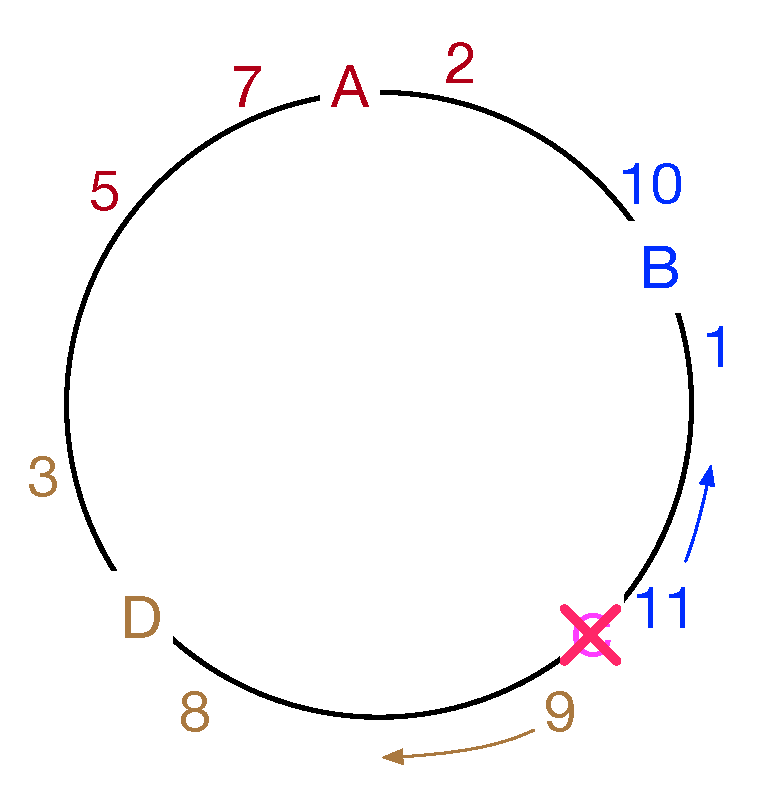
\includegraphics[width=\textwidth]{figures/consistent_hashing_3.eps}
\end{column}
\end{columns}

If a node fails, its neighbors consult all replicas of that node, to take over the documents that are now (temporarily) unavailable.

\end{frame}